\documentclass[a4paper,twoside]{book}

\usepackage[utf8]{inputenc}
%\usepackage[T1]{fontenc}
%\usepackage{times}
%\usepackage{utopia}
\usepackage{palatino}
%\usepackage{bookman}
\usepackage{fancyhdr}
\usepackage{multirow}
\usepackage{graphicx}
\usepackage{epstopdf}
\usepackage{sidecap}
%\usepackage{hyperref}
\usepackage[breaklinks=true]{hyperref}
\usepackage{verbatim} 
\usepackage{multirow, array, wrapfig}
\usepackage[disable]{todonotes}
\usepackage{pdfpages}
\usepackage{fixltx2e}
\usepackage{siunitx}

\hypersetup{
    pdftoolbar=true,        % show Acrobat’s toolbar?
    pdfmenubar=true,        % show Acrobat’s menu?
    pdffitwindow=false,     % window fit to page when opened
    pdfstartview={FitV},    % fits the width of the page to the window
    pdftitle={9th HGSFP Winter School 2016},    % title
    pdfauthor={},     % author
    pdfsubject={Workshop Program},   % subject of the document
    pdfcreator={},   % creator of the document
    pdfnewwindow=true,      % links in new window
    colorlinks=true,       % false: boxed links; true: colored links
    linkcolor= black,          % color of internal links (change box color with linkbordercolor)
    urlcolor= blue           % color of external links
}


\setlength{\topmargin}{0mm}
\setlength{\headheight}{14pt}
\setlength{\headsep}{10mm}
\setlength{\textwidth}{145mm}
\setlength{\textheight}{220mm}
\setlength{\evensidemargin}{4mm}
\setlength{\oddsidemargin}{7mm}

\addtolength{\headwidth}{+6mm}

% hier wird "Luft" gemacht :)
\renewcommand{\baselinestretch}{1.2}

\renewcommand{\thefootnote}{\fnsymbol{footnote}}

\newcommand{\chap}[1]{{\LARGE \bf #1}\\ \vspace{0.5 cm} \noindent}
% 


%\newcommand{\student}[9]{%
%	\ptitle{#6} \\%
%	\aauthor{#1} \\%(\href{mailto:#2}{\nolinkurl{#2}})\\%
%	\aaffiliation{}{#4}\\%	
%	#7 \\%
%}

\newcommand{\atitle}[1]{{\bf \large \centering #1 \\ \medskip}}
\newcommand{\aauthor}[1]{{\bf  \centering #1 \\ \bigskip}}
%\newcommand{\aaffiliation}[2]{\noindent \parbox[t][][t]{0.3cm}{\small #1} \parbox[t][][t]{13.6cm}{\small #2}\vspace{.2cm}\\}
\newcommand{\aaffiliation}[1]{{\noindent \small #1}\vspace{.2cm}}
\newcommand{\ptitle}[1]{{\bf \centering #1 \\ \medskip}}
\newcommand{\paffiliation}[1] {\noindent {\small #1} \\} 
\newcommand{\student}[9]{
    \begin{minipage}[t][0.49\textheight]{\textwidth}
		\ptitle{#8} 
		\aauthor{#1}
		\paffiliation{#4}
		\aaffiliation{Research Area: #6}
		
		#7
		
		\vspace*{0.6cm}
    \end{minipage} \\
}

\begin{document}

\fancyhead{} % clear all header fields
\fancyfoot{} % clear all footer fields
\fancyfoot[LE,RO]{\thepage}
\fancyfoot[LO,RE]{10th HGSFP Winter School 2017}
\renewcommand{\headrulewidth}{0.4pt}
\renewcommand{\footrulewidth}{0.4pt}


\pagestyle{empty}

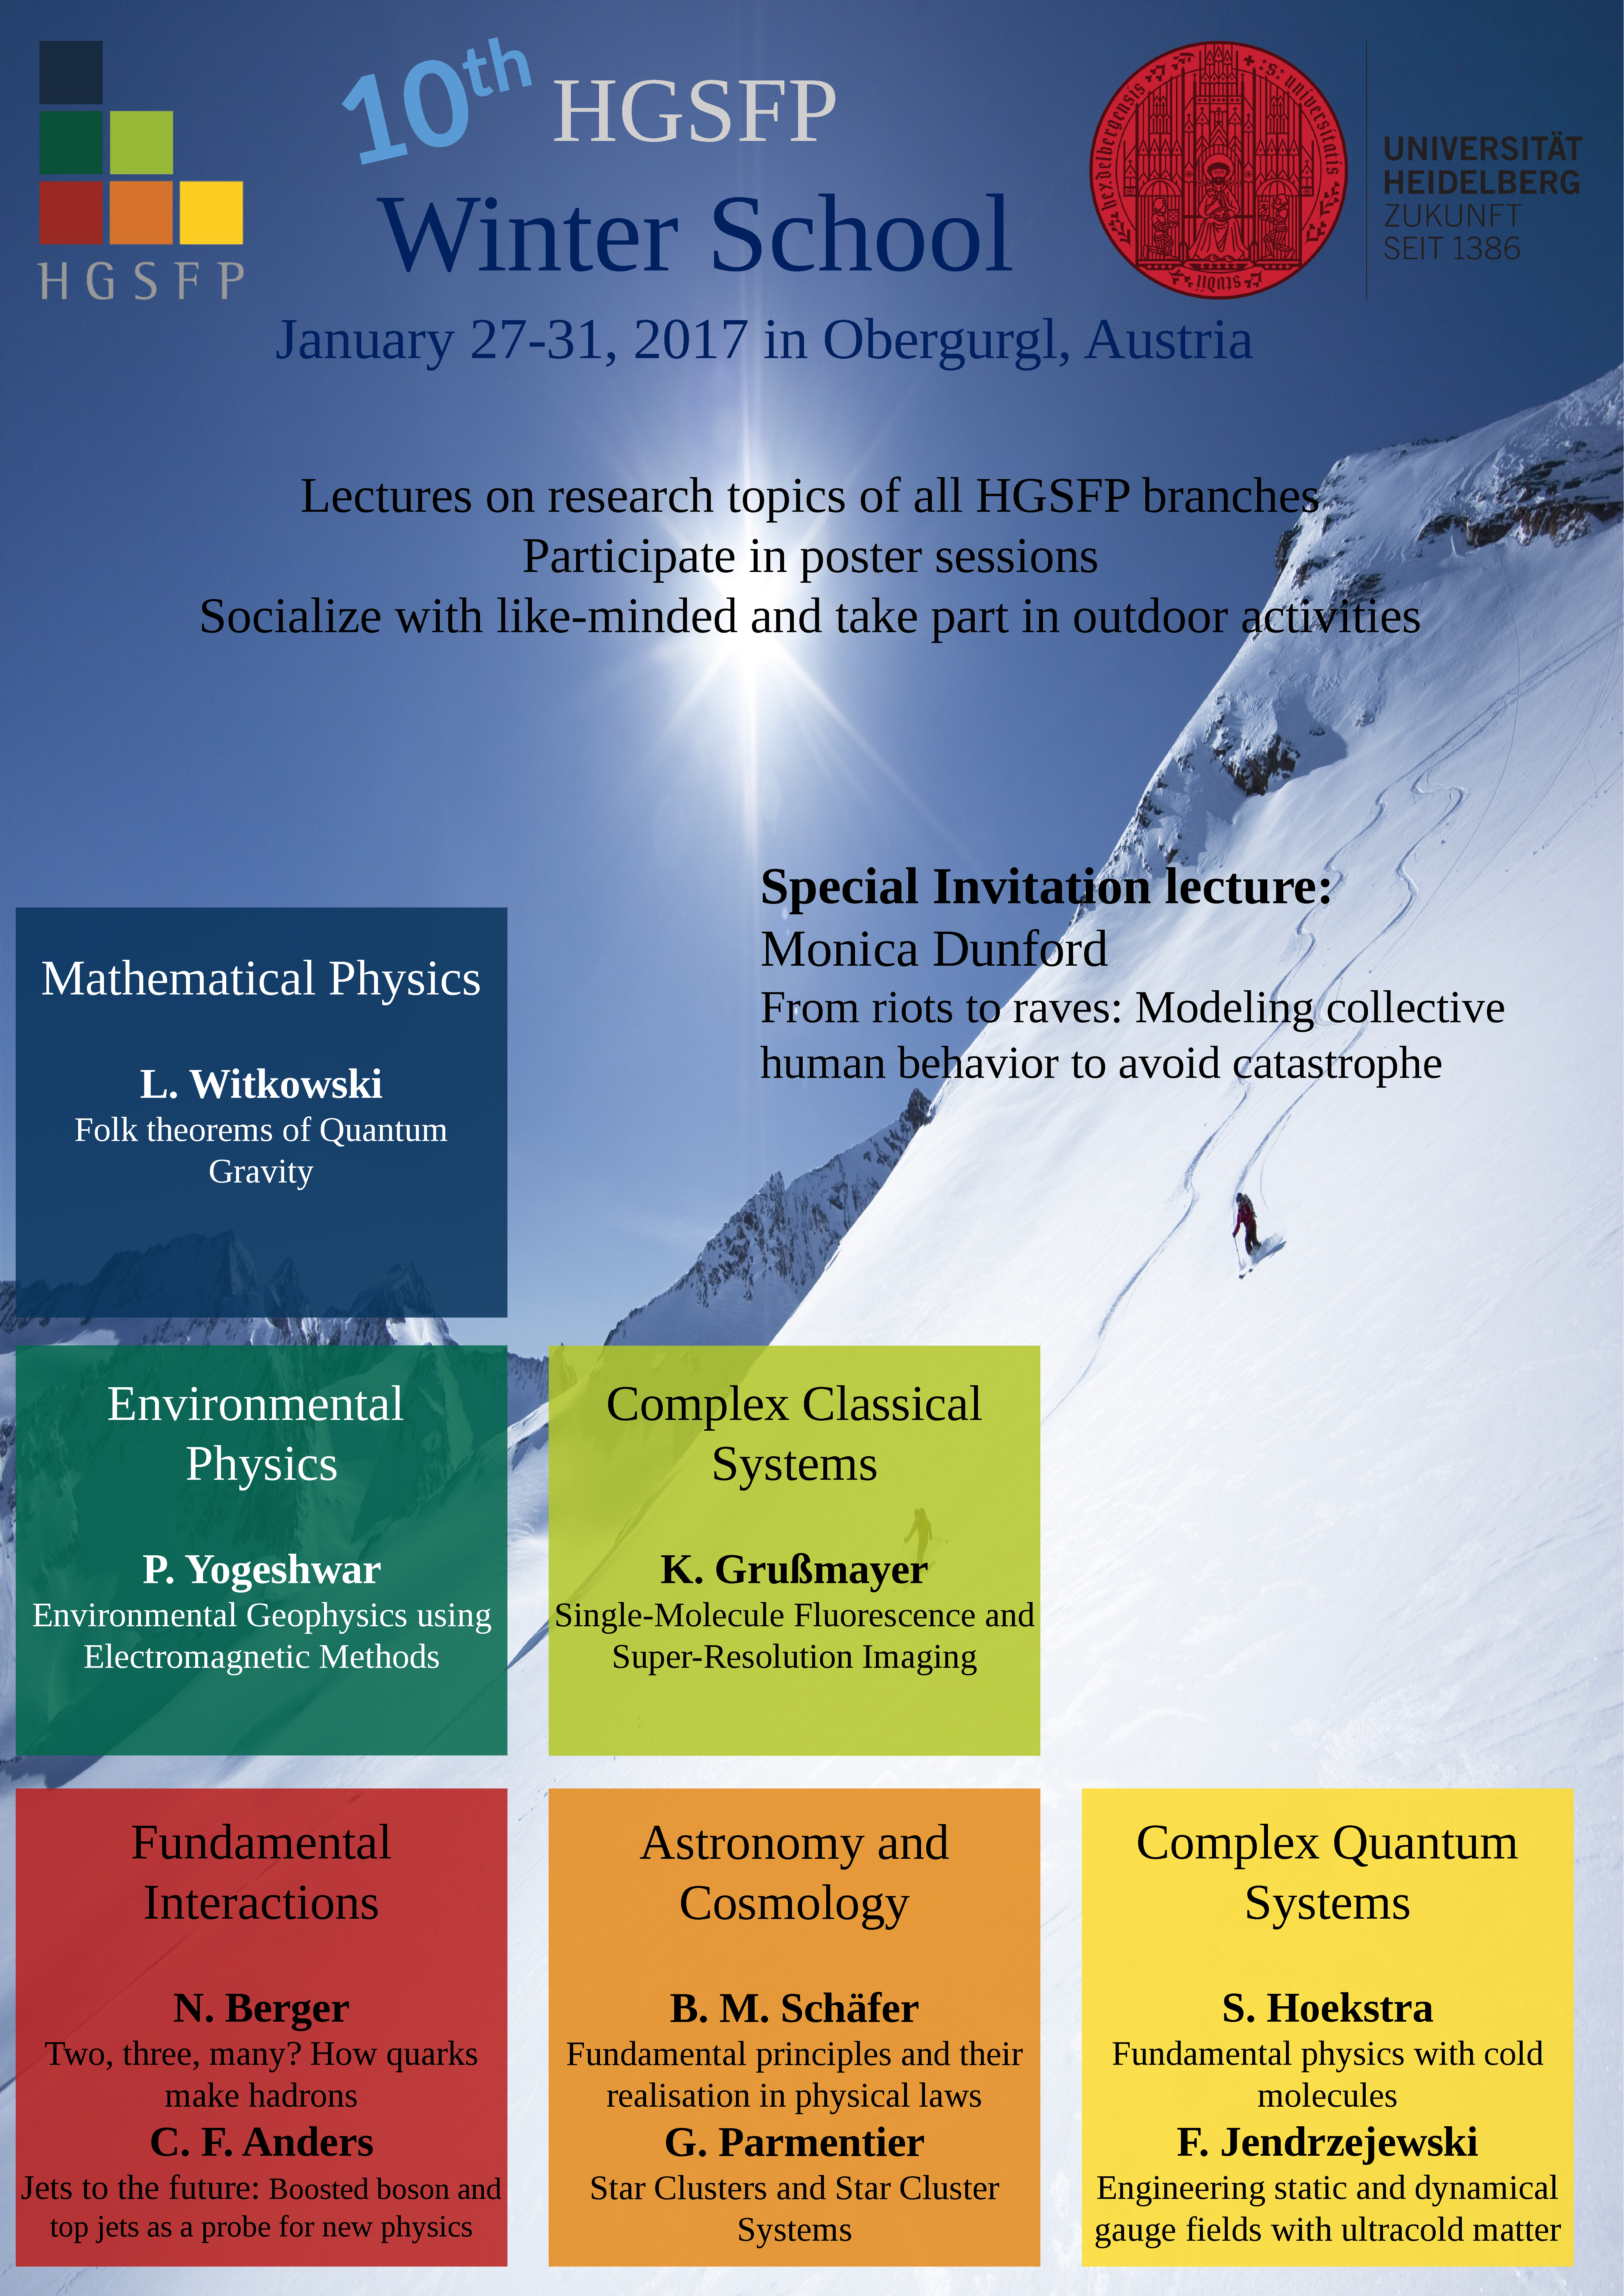
\includepdf{Booklet_front_page.pdf}

\cleardoublepage


\noindent
{\Huge 10th HGSFP Winter School 2017}

\vspace{1cm}
\noindent
{\Large January 27 - 31, 2016 \\ Universit\"atszentrum Obergurgl}

\vspace{4cm}
\noindent
{\Large Book of Abstracts and Workshop Program}


\vspace{8cm}

\noindent
\begin{tabular}{b{9cm}}
	{\bf Organisation:}\\
	Heiko Augustin \\
	David Gerick \\
	Lennart Huth \\
	Frank Könnig \\
	Janko Nauta \\
	Merve Şahinsoy \\
\end{tabular}


\vspace{1cm}

\noindent
\begin{tabular}{b{9cm} p{3cm} b{4cm}}
	& & \multirow{3}{*}{
\includegraphics[scale=0.18]{hgsfp.eps}} \\ 
	{\bf Acknowledgements: } \\
	This school has been made possible by the \\ 
	Heidelberg Graduate School for Fundamental Physics. \\
\end{tabular}

%\newpage
%\tableofcontents

\makeatletter
\@openrightfalse
\tableofcontents
\@openrighttrue
\makeatother

\pagenumbering{arabic}
\pagestyle{fancy}

\clearpage
\fancyhead[RO,LE]{\bfseries General information}
%\input{generalinformation}

\clearpage 
\fancyhead[RO,LE]{\bfseries Schedule}
\addcontentsline{toc}{section}{Program and Events}

\noindent
\chap{Program and Events}

\subsection*{Thursday, 26\textsuperscript{th} of January}

\begin{tabular}{p{2.5cm}p{11.5cm}}
	23:30 & Departure from Heidelberg \\
\end{tabular}

\subsection*{Friday, 27\textsuperscript{th} of January}

\begin{tabular}{p{2.5cm}p{11.5cm}}
	ca. 7:00 & Arrival in Obergurgl \\ 
	at arrival & Breakfast (provided) \\ 
	until diner & free afternoon \\
	18:00 & Dinner (provided) \\
	20:00 & Social event \\
\end{tabular}

\subsection*{Saturday, 28\textsuperscript{th} of January - Monday, 30\textsuperscript{th} of January}

\begin{tabular}{p{2.5cm}p{6cm}}
	7:30 & Breakfast (provided) \\
	8:30 - ca. 10:15 & Lecture \\ 
	\cline{1-2}
	Lunchbreak \\
	\cline{1-2}
	17:00 - ca. 18:45 & Lecture \\ 
	19:00 & Dinner (provided) \\
	20:00 & \textbf{Saturday} Elevator talks session I \\
		  & \textbf{Sunday}  Elevator talks session II \\
		  & \textbf{Monday} Introduction to the HGSFP \\
	20:30 & \textbf{Saturday} Poster session I \\
		  & \textbf{Sunday}  Poster session II \\
		
\end{tabular}

\subsection*{Tuesday, 31\textsuperscript{th} of January}

\begin{tabular}{p{2.5cm}p{6cm}}
	7:30 & Breakfast (provided) \\
	8:30 - ca. 10:15 & Lecture \\ 
	\cline{1-2}
	Lunchbreak \\
	\cline{1-2}
	16:00 & Departure from Obergurgl \\ 
\end{tabular}
\vfill

\noindent

\begin{figure}
  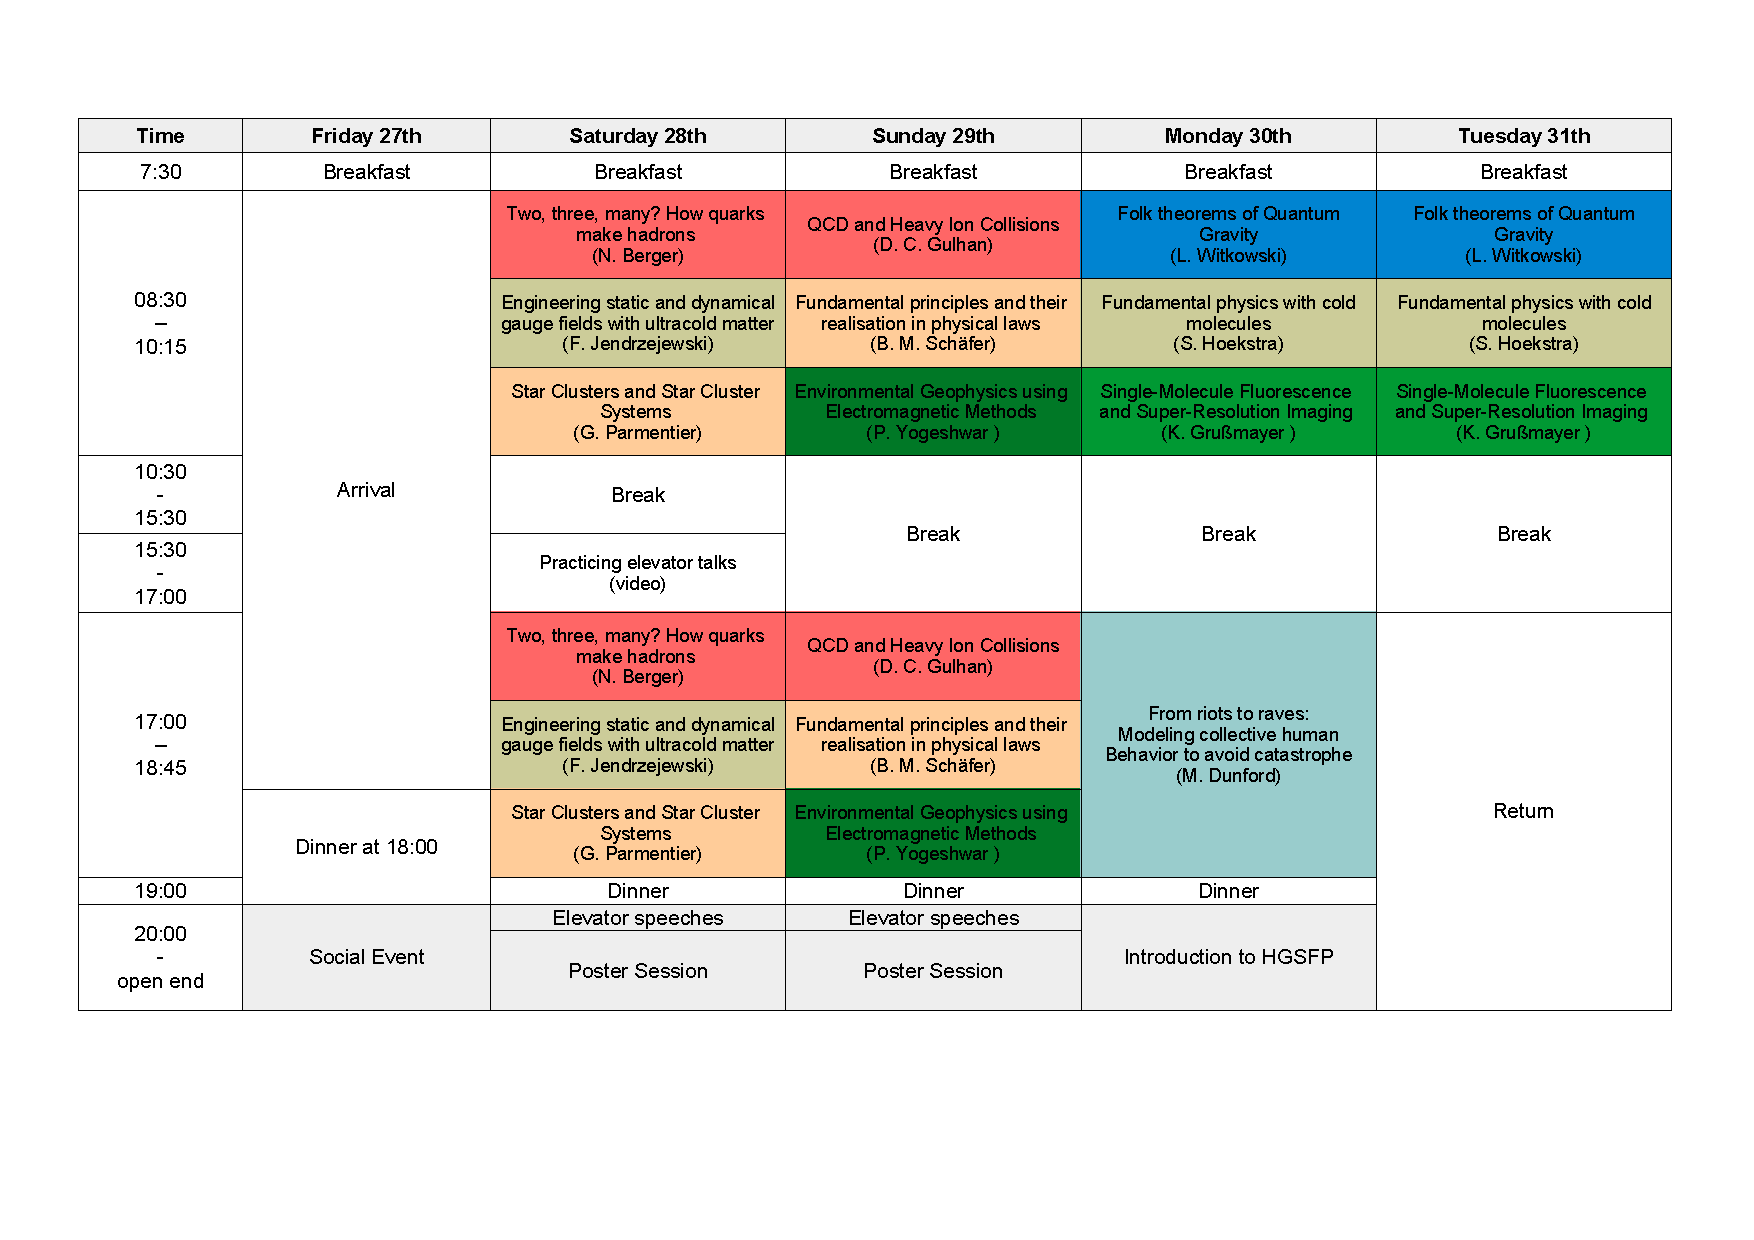
\includegraphics[angle = 90,width=1.1\textwidth]{FinalProgram}
\end{figure}


\clearpage
\addcontentsline{toc}{section}{Lectures}
\fancyhead[RO,LE]{\bfseries Lectures}
\noindent

\chap{Lectures}
\subsection*{Two, three, many? How quarks make hadrons}
\subsection*{N. Berger, Uni Mainz}
\noindent What are the bound states of the strong interaction? Is there something beyond meson (quark-antiquark) and baryon (three quark) states? Recent discoveries, especially in the charm quark sector, challenge our understanding of the bound states of the strong interaction. The lecture discusses these discoveries and the attempts at theoretical understanding, giving insights into a rapidly changing field of particle physics. 
\clearpage
\subsection*{Single-Molecule Fluorescence and Super-Resolution Imaging}
\subsection*{K. Gru\ss mayer, Ecole Polytechnique Fédérale de Lausanne}
\noindent 
“A biological system can be exceedingly small. Many of the cells are very
tiny, but they are very active; they manufacture various substances; they walk
around; they wiggle; and they do all kinds of marvelous things – all on a very
small scale.” R. P. Feynman (1959)\newline

Light microscopy is one of the most important methods to investigate the
structure and function of (living) biological systems. These are ultimately
based on the dynamics and interactions of individual molecules. In the last
decades, developments in experimental physics along with advances in
(bio-)chemistry were the driving force that allowed investigating those
processes at the molecular level. I will concentrate on fluorescence imaging,
which is ideally suited to study single-molecules due to its sensitivity. I
will introduce important milestones in this young field, along with the major
microscopy techniques, photophysical processes and statistical analysis
required to obtain quantitative information.  In the second part of the
lecture, I will focus on how the properties of fluorophores along with a
clever optical design can be used to overcome Abbe’s diffraction limit of
light microscopy. For their “development of far-field super-resolved
microscopy”, three physicists were awarded the Nobel Prize in Chemistry
2014. I will discuss how the techniques can be pushed to reach the limits – a
spatial resolution approaching the size of single-molecules. 
\clearpage
\subsection*{QCD and Heavy Ion Collisions}
\subsection*{D. C. Gulhan, CERN}
\noindent
\clearpage
\subsection*{Fundamental physics with cold molecules}
\subsection*{S. Hoekstra, Uni Groningen}
\noindent Atomic and molecular physics has in recent years seen an strong evolution on two experimental fronts: the exquisite control over atomic and molecular samples, and the availability of extremely stable laser light over a wide frequency range. By combining these experimental precision tools with theory that explains atomic and molecular structure at a similar level of precision, a powerful field has emerged, providing a new perspective on the fundamental interactions and symmetries of our universe. Of special interest are the developments on cooling of molecules, which through huge enhancement effects are promising superior sensitivity. By combining precision table-top experiments, quantum structure calculations and particle-physics theory, the understanding of the foundations of our universe can be tested at energies that effectively surpass those available at the largest particle accelerators that have been built. In these lectures, I will give an overview of the main concepts and techniques in the field of cold molecules, especially where they are used to search for new physics.
\clearpage
\subsection*{Engineering static and dynamical gauge fields with ultracold matter}
\subsection*{F. Jendrzejewski, Uni Heidelberg}
\noindent
Gauge field dynamics have attracted considerable interest over the last few
years. In this course, we
will discuss the experimental tools that enabled the precise study of such
systems with ultracold
matter. First, we look into the techniques that enabled the study of static
gauge fields, similar to
actual magnetic fields, with neutral atoms. Then we will move on the
challenges to extend the
approaches to dynamical gauge fields, which would allow for the quantum
simulation of high-
energy problems and finally discuss first experimental results.
\clearpage
\subsection*{Star Clusters and Star Cluster Systems}
\subsection*{G. Parmentier, Uni Heidelberg}
\noindent Clusters of stars represent a major channel of star formation and
hold therefore the potential to trace the star formation history of galaxies.
There is still a long way to go before reaching that goal, however.
Firstly, a significant fraction of the star clusters of any galaxy remains
undetected.  Secondly, star clusters 'dissolve' (i.e. they lose stars) as time
goes by, at a rate depending on both cluster formation and
environmental conditions.  Building on the cluster age-mass diagram and
on a cluster formation model, I will illustrate these two issues. 
\clearpage
\subsection*{Fundamental principles and their realisation in physical laws}
\subsection*{B. M. Sch\"afer, Uni Heidelberg}
\noindent This course is intended to be guided discussion about fundamental principles and how they are realised in classical and modern physics. We will discuss hidden and implicit assumptions in basic formalisms and talk about (hopefully unusual) approaches to modern physics, in particular the construction of field theories including general relativity and electrodynamics. We will conclude with a discussion of general relativity in everyday life - and I’m serious about this.
\clearpage
\subsection*{Folk theorems of Quantum Gravity}
\subsection*{L. Witkowski}
\noindent
\clearpage
\subsection*{Environmental Geophysics using Electromagnetic Methods}
\subsection*{P. Yogeshwar, University of  Cologne}
\noindent
Geoelectrical and electromagnetic geophysical techniques have become very popular for various environmental applications such as for example groundwater exploration/management, investigation of waste disposal sites and detection of suitable landfills. These surface geophysical methods are non-invasive and provide valuable information of the subsurface physical properties. The resolved physical parameter (e.g rock density, magnetic susceptibility and electrical conductivity) depends on the applied geophysical exploration technique. Geoelectrical and electromagnetic methods are sensitive to the subsurface electrical conductivity. The electrical conductivity spans approximately 25 decades of magnitude for materials occurring in the earth's subsurface. Massive dry rocks exhibit extremely low electrical conductivities and are nearly transparent for electromagnetic methods, whereas for example a contaminated aquifer due to saline water intrusion serves as a suitable target. Due to the close relationship between electrical conductivity and (some) hydrogeological properties of aquifers, geoelectrical and electromagnetic techniques are the most popular in groundwater exploration.\\
The first part of this lecture gives a brief overview of geoelectrical and electromagnetic geophysical methods with respect to their typical areas of application, advantages/disadvantages and the different subsurface electrical conductivity mechanisms. The second part focuses comprehensively on the transient electromagnetic method (TEM) using mainly inductively ground-coupled loop sources. The TEM method has gained extreme popularity for environmental targets in the past decades and is commonly used for groundwater exploration. The lecture discusses various important aspects with respect to the TEM method, namely: basic methodological concepts, common measurement devices, typical TEM survey layouts, general noise-sources and coupling effects, processing techniques, interesting TEM source-field modifications and, finally, the conventional forward and inverse modeling techniques to reconstruct the subsurface electrical conductivity distribution. In the third part, recent real-world case studies are comprehensively discussed. A focus lies on an exemplary study from the Azraq Basin area. This area is of enormous economical importance to Jordan. Approximately one third of the freshwater for Jordan’s capital city of Amman is provided from the Azraq area. The extensive groundwater exploitation has led to a severe decline in the groundwater table. In the central part of the area, the groundwater is hyper-saline. To ensure the freshwater supply, groundwater research has been (and still is) an ongoing and relevant issue over the past 30 years. The presented geophysical investigations provide information about the extent of the saline water body and aim to support the ongoing groundwater management in the area.
\clearpage

\clearpage
\addcontentsline{toc}{section}{General Lecture} 
\fancyhead[RO,LE]{\bfseries General Lecture}
\noindent
\chap{General Lecture}

\subsection*{From riots to raves: Modeling collective human behavior to avoid catastrophe}
\subsection*{Monica Dunford, Uni Heidelberg}
\noindent Why do some protests become riots and others stay peaceful? What
triggers a crowd to panic resulting in people being trampled to death?
Understanding collective human behavior and motion is critical to prevent
future crowd catastrophes. This lecture will discuss models that attempt to
predict the behavior of crowds with high emotional intensity and often
alcohol, drugs and weaponry. 


\clearpage
\addcontentsline{toc}{section}{Student poster abstracts} 
\fancyhead[RO,LE]{\bfseries Student poster abstracts}
\noindent

\newpage
\thispagestyle{empty}
\vspace*{0.4\textheight}
%\centering
{\LARGE \bf Student poster abstracts }
%\chap{Student poster abstracts}\\
%
%\vspace{-3cm}%
\newpage 
\noindent
\subsection*{\centering \large M54: A key for the connection between globular and nuclear star clusters}
\subsection*{\centering \normalsize Alfaro Cuello, Mayte}
Research Area: Nuclear Star Clusters and Black Holes\newline

\noindent M54 is the second most massive stellar cluster in the Milky Way. It shows
a large iron abundance spread in its stars, a kinematic signature for a
massive black hole at its center (104Msol) and it is thought to be the
stripped nuclear star cluster of the accreted Sagittarius dwarf galaxy.
These facts and its proximity (26.8 kpc) make M54 an ideal laboratory for
studying the still unknown connection between globular and nuclear star
clusters. We present a large MUSE data set (3.25"x3.25") covering ~2.5Reff
of this stellar cluster, from which spectral and kinematic information can
be extracted for a large number of stars. With these data we will be able
to connect the spatial information to kinematics and element abundance
measurements, allowing us to constrain the formation history of M54. This
may pave the way to uncover the origin of the most massive globular
clusters in the Milky Way.
\subsection*{\centering \large Neutrino detection efficiency in the Double Chooz experiment}
\subsection*{\centering \normalsize Almazan Molina, Helena}
Research Area: Reactor neutrino physics \newline

\noindent Nuclear reactors are an intense and pure source of low energy electron antineutrinos, being one of the most powerful tools to investigate neutrino oscillations. The Double Chooz experiment aims for a precise determination of the neutrino mixing angle $\theta_{13}$ using a two detector configuration with a liquid scintillator target volume read by photomultipliers. \\The antineutrino detection efficiency systematic uncertainty is the dominant component in the normalization uncertainty affecting the final precision on the $\theta_{13}$ measurement. The collected data from the near detector since January 2015 will profit from improved detection systematic uncertainties thanks to the cancellation of correlated contributions.
\newpage
\subsection*{\centering \large Commissioning of a saturated algorithm in the ATLAS Level-1 Calorimeter Trigger}
\subsection*{\centering \normalsize Antel, Claire}
Research Area: Dark Matter searches in dijet events with ATLAS\newline

\noindent Proton-proton collisions at the Large Hadron Collider (LHC) are of unprecedented high instantaneous luminosity. The first step to recording these collision events at the ATLAS experiment is performing an ultrafast analysis of the collision to quickly and effectively sieve out all but the most interesting events for physics which are to be processed more carefully.\\The ATLAS Level-1 trigger is required to perform this essential job within 2.5 microseconds. Processes that occur within this time are, amongst others, digitization of analogues signals, digital to particle energy conversion and bunch crossing identification. Misidentifying the bunch crossing will lead to the event being irrevocably lost.\\A new algorithm was commissioned for the level-1 trigger in ATLAS for the current physics data taking period, which is designed to identify the bunch crossing of a collision for saturated pulses and is suited for the record-breaking proton collision energies the LHC is currently running at. \\The algorithm was enabled towards the end of the 2016 physics data taking period. Its 

 

\subsection*{\centering \large The MuPix7}
\subsection*{\centering \normalsize Augustin, Heiko}
Research Area: Muon physics \newline

\noindent The search for new physics at low energy requieres high sensititivty to rare proccesses and opens an alternative way compared to large collider experiments. Therefor, new detector concepts are used. One decay of interest is the decay of a muon into three electrons. This decay is cLFV and heaviely suppressed in the SM. Any obersevation is a clear sign for new physics. The Mu3e experiment aims to find or exclude this decay down to a BR of $10^{-16}$. I work on the development of the tracker, which includes R\& D in the field of HV-MAPS, readout and slow control.
\newpage

\subsection*{\centering \large Aircraft-based 2- and 3D Measurements of Trace Gas Emissions of Megacities}
\subsection*{\centering \normalsize Bigge, Katja}
Research Area: Bestimmung der zwei- und dreidimensionalen Verteilung von Spurengasen mit dem Heidelberger Abbildendes Flugzeug-DOAS Instrument (HAIDI) auf HALO\newline

\noindent While trace gases only account for a miniscule percentage of the atmospheric composition,they play an important role for chemical processes, thermal structure and other basic characteristics. Remote sensing can allow for a comprehensive probing of their distribution.While satellite instruments have excellent spatial coverage, their spatial and temporal resolution is low.Also, in the vertical dimension, no or very low spatial resolution is available.On the other hand, aircraft-based instruments can achieve a high spatial and temporal resolution during overflight. The Heidelberg Airborne Imaging DOAS Instrument (HAIDI) was developed to survey distributions of trace gases in 2D and 3D.During the EMerGe (Effect of Megacities on the Transport and transformation of Pollutants on the Regional to Global Scales) mission of the research aircraft HALO,it will be dispatched to investigate the outflow of megacities and the atmospheric impact of urban pollution. The combination of advanced viewing geometry and high signal-to-noise ratio due to very high instrumental light,the reconstruction of the spatial distribution of trace gases and\\aerosols will be possible using novel retrieval algorithms.

\subsection*{\centering \large A new electron beam ion source as charge breeder for rare isotope beams}
\subsection*{\centering \normalsize Blessenohl, Michael}
Research Area: \newline

\noindent TRIUMF as Canadian national research facility operates the largest cyclotron in the world, which accelerates protons to $500\,\textrm{MeV}$. These high-energy protons are sent to a target composed of heavy elements which on impact produces heavy isotopes to be studied in the two post-accelerators ISAC (Isotope Separator and Accelerator) I and ISAC II.\\The new ARIEL (Advanced Rare IsotopE Laboratory) at TRIUMF will include a new electron beam ion source (EBIS) for charge breeding [1] these rare isotope beams. Highly charged heavy elements are used to keep the charge to mass ratio $\kern.1em\raise.5ex\hbox{\the\scriptfont0 A}\kern-.1em/\kern-.15em\lower.25ex\hbox{\the\scriptfont0 Q}$ low, which is required by the post-accelerators ISAC I and II. Aiming at the studies of isotopes with half-lives down to $65$\,milli\-seconds and low abundances of down to $10^6$ per bunch, the whole process of injection, charge breeding and extraction has to be very efficient. The repetition rate of the isotope bunches is $100\,\textrm{Hz}$, which requires fast high-voltage control and switching. The goal is to have a charge breeding efficiency of at least $20\,\%$.\\Here the latest design is presented, including finite-element and Monte-Carlo simulation results, concepts for the on-line diagnostics and a fast control system.
\newpage
\subsection*{\centering \large Testing CPT Symmetry Through Precision g-Factor Measurements}
\subsection*{\centering \normalsize Bohman, Matthew}
Research Area: Precision Measurements of the Proton Magnetic Moment\newline

\noindent Charge-Parity-Time (CPT) symmetry is believed to be one of the fundamental symmetries of nature, however, the Standard Model, with an unbroken CPT symmetry does not explain the observed baryonic asymmetry. Precision measurements to the ppb or ppt and beyond will prove essential to understanding this phenomenon. In fact, measurements of the proton and anti-proton g-factor in Penning traps currently allow for some of the most stringent tests of CPT symmetry violation. In both experiments a ???double-trap??? technique allows for high fidelity read out of the spin state and high precision measurement of the trapped particle eigenfrequencies.
\subsection*{\centering \large Measuring $|V_{ub}|$ at LHCb}
\subsection*{\centering \normalsize Braun, Svende}
Research Area: Particle Physics \newline

\noindent Precise measurements of the quark coupling strength allow a strong test of the unitarity of the CKM matrix. $|V_{ub}|$ is the least well known CKM element and previous measurements using exclusive and inclusive methods have resulted in values of $|V_{ub}|$ which are 3$\sigma$ apart. The first measurement of $|V_{ub}|$ at LHCb confirmed this tension using the $\Lambda^0_b \rightarrow p \mu^- \bar{\nu}$ decay. This strengthens the motivation to measure this quantity using different channels. With recent lattice QCD calculations, LHCb can also constrain $|V_{ub}|$ using the $B^0_s\rightarrow K^+ \mu^- \bar{\nu}$ decay where the theoretical uncertainty is significantly smaller.

\newpage
\subsection*{\centering \large Direct Imaging of Exoplanets with NaCo-ISPY}
\subsection*{\centering \normalsize Brems, Stefan}
Research Area: Direct Imaging of Exoplanets with NaCo-ISPY\newline

\noindent One of the fastest growing fields in astronomy during the last years is the field of Extrasolar Planets, or short Exoplanets. There is various methods to detect those, each coming with different advantages and disadvantages. The NaCo-ISPY program being presented uses the direct imaging technique, meaning one tries to find and characterise new planets by literally taking pictures of the Exoplanet orbiting its hoststar. The first data was taken in December 2015 and the search will continue until about 2020 with the NaCo instrument at the Very Large Telescope (VLT) in Chile. This poster will present the technique of high contrast imaging as well as the results we got so far.


\subsection*{\centering \large The clumpy nature of star formation in NIHAO}
\subsection*{\centering \normalsize Buck, Tobias}
Research Area: Milky Way simulations\newline

\noindent Many massive star forming disk galaxies in the redshift range 3 to 0.5 are observed to have a clumpy morphology with giant clumps of size $\sim$1 kpc and masses of about $10^8$~Msun to $10^{10}$~Msun. The nature and fate of these giant clumps is still under debate. Some previous theoretical studies found that giant clumps are self-bound, long-lived structures that spiral inwards and influence strongly the evolution of the host galaxy and especially contribute to the bulge formation while other studies found that clumps do not contribute to the bulge growth and are disrupted quickly by stellar feedback processes. In this work we present results derived from the largest sample of homogeneous high-resolution simulations which were run down to redshift zero producing galaxies with realistic properties. We are using 19 high-resolution simulations of disk galaxies from the NIHAO sample to study giant clumps and their influence on galaxy morphology. We use all galaxies with stellar masses greater than $M_{*}\sim10^{9.5}$~Msun at redshift 1.5. We apply an observationally motivated clump selection and pick clumps as local maxima in the U-band luminosity images of the galaxies. Selecting U
\newpage
\subsection*{\centering \large Scalar-tensor theories in the non-linear regime}
\subsection*{\centering \normalsize Casas, Santiago}
Research Area: \newline

\noindent Abstract We forecast parameters of modified gravity theories that affect the Poisson equation and the anisotropic stress of General Relativity and focus on the non-linear regime.

\newpage
\subsection*{\centering \large Possible explanation for the `Dark Matter X-ray line' at $\sim 3.5\,\mathrm{keV}$ by
charge exchange between  $\mathrm{S}^{16+}$ and neutrals}
\subsection*{\centering \normalsize Dobrodey, Stepan}
Research Area: Charge breeding of rare, short lived isotopes\newline

\noindent Speculations about a possible dark matter origin of a weak x-ray transition at $\sim 3.5\,\mathrm{keV}$ have attracted enormous attention in the scientific community. A cautious explanation was recently given by Gu et al.: charge exchange (CX) between fully stripped sulfur and atomic hydrogen.
By populating states in high principal quantum numbers $n_{\mathrm{cx}}$ of $\mathrm{S}^{16+}$, the process drives a radiative cascade directly feeding the $n = n_{\mathrm{cx}}$ to $n = 1$ transitions. We approach the problem experimentally by breeding $\mathrm{S}^{16+}$ ions in FLASH-EBIT and keeping them magnetically confined with the electron beam turned off. During recombination of those ions with residual gas we collect x-ray spectra with a resolution of FWHM $\sim 150\,\mathrm{eV}$. The $3.5\,\mathrm{keV}$ transition shows clearly up in the spectra under a wide variety of conditions and agrees with the astrophysical observations and the predictions of Gu and Kaastra.

\subsection*{\centering \large The ALPHATRAP g-Factor Experiment}
\subsection*{\centering \normalsize Egl, Alexander}
Research Area: g-factor measurements on highly charged ions\newline

\noindent The Penning-trap experiment ALPHATRAP at the Max-Planck-Institut f\""ur Kernphysik is currently being set up and aims to test bound-state quantum electrodynamics by determining the \textit{g}-factor of the bound electron in the electric field of heavy highly-charged ions (HCI) with ultra-high precision, similar as already done at the University of Mainz on light systems like $^{12}\textrm{C}^{5+}$,$^{28}\textrm{Si}^{13+}$ and $^{40,48}\textrm{Ca}^{17+}$. \\To achieve this, the ALPHATRAP experiment consists of an open cryogenic double Penning-trap setup. The double Penning trap is coupled via an ultra-high vacuum beamline to the Heidelberg Electron-Beam Ion Trap (Heidelberg-EBIT), which provides the HCI up to hydrogen-like $^{208}\textrm{Pb}^{81+}$. ALPHATRAP will be the first Penning-trap experiment employing sympathetic laser-cooling to the stored highly-charged ions for \textit{g}-factor measurements.\\Therefore a setup for the creation and Doppler laser cooling of $^{9}\textrm{Be}^{1+}$ is in development.\\An overview and the current status of the project will be presented.

\newpage
\subsection*{\centering \large Using reverberation mapping to determine the composition of Active Galactic Nuclei}
\subsection*{\centering \normalsize Esser, Johannes}
Research Area: AGN dust reverberation mapping\newline

\noindent The unified model of Active Galactic Nuclei (AGN) gives a good explanation how different features and viewing angles lead to the appearances of AGN. AGN are made up of a supermassive black hole accreting mass, a dusty torus blocking the view from certain viewing angles and gaseous clouds within the torus (the so called broad line region) and above the torus (the narrow line region). However the origin of the different features is still unknown. We are not able to make direct images of AGN, because of the distance and size of AGN. Fortunately all features of the AGN are illuminated by the accretion disc in the center of the AGN. Therefore luminosity changes of the accretion disc are followed by luminosity changes of the other components. These delays correspond to the light travel time to the center of the AGN and a map of the AGN can be made. Moreover we investigate changes of the broad line region to determine the origin of the fast moving gas clouds close to the center of the AGN.

\subsection*{\centering \large Simulating many-body spin dynamics with Rydberg atoms}
\subsection*{\centering \normalsize Ferracini Alves, Renato}
Research Area: Simulation of spin dynamics using Rydberg atoms\newline

\noindent Simulating many-body spin-dynamics is of great interest both for its connection to practical systems, such as quantum magnetism, spintronics, and polar molecules [1], as well as for getting a deeper insight in systems driven by a many-body Hamiltonian. In our experiment we realize a Heisenberg XX-model by mapping two dipolar-interacting Rydberg states to two spins states (|nS??????|?????? and |nP??????|??????). This scheme allows us to explore the dynamics of spin systems with long range interactions [2].\\We will present preliminary results of the measurement of microwave-driven Rabi oscillations between the spin-states, in which interactions lead to damping of the contrast for high Rydberg densities [3].\newline [1] B. Yan et al., Nature 501, 521-525 (2013) \newline [2] D. Barredo et al., Phys. Rev. Lett. 114. 113002 (2015) \newline [3] D. Maxwell et al., Phys. Rev. Lett. 110, 103001 (2013)


\newpage
\subsection*{\centering \large Purely flavor-changing $Z^\prime$ and where it might hide}
\subsection*{\centering \normalsize Foldenauer, Patrick}
Research Area: \newline

\noindent A plethora of ultraviolet completions of the Standard Model have extra U(1) gauge symmetries. In general, the associated massive $Z^\prime$ gauge boson can mediate flavor-changing neutral current processes at tree level. We consider a situation where the $Z^\prime$ boson couples solely via flavor-changing interactions to quarks and leptons. In this scenario the model parameter space is, in general, quite well constrained by existing flavor bounds. However, we argue that cancellation effects shelter islands in parameter space from strong flavor constraints and that these can be probed by multi-purpose collider experiments like ATLAS or CMS as well as LHCb in upcoming runs at the LHC. In still allowed regions of parameter space these scenarios may help to explain the current tension between theory and experiment of $(g-2)_\mu$.

\subsection*{\centering \large From dwarf galaxies to satellites}
\subsection*{\centering \normalsize Frings, Jonas}
Research Area: Simulations of Milky Way Satellites \newline

\noindent We study the effect of stripping of satellite galaxies in Milky Way mass halo by starting with 7 cosmological zoom in simulations of dwarf galaxies in the halo mass range $5\cdot10^8\,M_\odot$ to $10^10\,M_\odot$, cutting them from the cosmological simulation at $z=1$ and study their evolution as a satellite galaxy by placing them on a realistic orbit in Milky Way potential with a ram pressure model. Our results indicate that the central dark matter density can drastically decrease in a few pericenter passages while the inner slope of the dark matter density profile is not strongly affected.

\newpage
\subsection*{\centering \large Photon production during the early stages of a Heavy Ion Collision}
\subsection*{\centering \normalsize Garcia Montero, Oscar}
Research Area: Non-equilibrium QCD\newline

\noindent We compute the cross section for photons emitted from sea quarks in proton-nucleus collisions at collider energies. The computation is performed within the dilute-dense kinematics of the Color Glass Condensate (CGC) eective eld theory. Albeit the result obtained is formally at next-to-leading order in the CGC power counting, it provides the dominant contribution for central rapidities. We observe that the inclusive photon cross section is proportional to all-twist Wilson line correlators in the nucleus. These correlators also appear in quark-pair production; unlike the latter, photon production is insensitive to hadronization uncertainties and therefore more sensitive to multi-parton correlations in the gluon saturation regime of QCD. We demonstrate that k? and collinear factorized expressions for inclusive photon production are obtained as leading twist approximations to our result. In particular, the collinearly factorized expression is directly sensitive to the nuclear gluon distribution at small x. Other results of interest include the realization of the Low-Burnett-Kroll soft photon theorem in the CGC framework and a comparative study of how the photon amplitude is obtained in Lorenz and light-cone gauges.

\subsection*{\centering\normalsize The participants of the HGSFP Winterschool 2017}
\subsection*{\centering\normalsize Gerick, David}
Research Area: Phd student statistics \newline

\noindent The 10th HGSFP Winterschool in Obergurgl welcomes exactly 50 students this year. The poster shows different statistics about the participants. The field of research, duration of study, the students' age and other statistics around the participants are shown. Furthermore, it shows the average PhD student participating in the school. All data is treated and shown anonymously.
\newpage

\subsection*{\centering \large Advancements and Prospects in Quantum Cascade Laser-based Glucose Monitoring}
\subsection*{\centering \normalsize Haase, Katharina}
Research Area: \newline

\noindent People suffering from Diabetes Mellitus, a metabolic disease of the pancreas, need to frequently measure their glucose concentration in order to prevent short and long term complications. We discuss different approaches to non-destructive and reagent free measurement of glucose concentration based on quantum cascade laser (QCL)-based mid-infrared (mid-IR) spectroscopy. Based on QCLs, one of the main challenges in mid-IR spectroscopy in vivo - the high absorption coefficient of water ??? can be overcome and a continuous glucose monitoring is possible. We assess the applicability of the different QCL-based approaches for usage in continuous and conceivable long term glucose measurements in patients.

\subsection*{\centering \large Ultrafast Exciton Dynamics in Diindenoperylene Films}
\subsection*{\centering \normalsize H\"ansel, Marc}
Research Area: Second Harmonic Generation at Photocromic Molecules and Donor Acceptor Interfaces\newline

\noindent Diindenoperylene (DIP) is a very promising material for organic electronics. It shows a high charge-carrier mobility, forms thin films with high structural order and is resistant to most environmental influences. In a photovoltaic device it can be used as donor or acceptor material. In this work we monitored the ultrafast (sub picosecond) excited states dynamics in (DIP) after optical excitation using time-resolved second harmonic generation (TR-SHG). We investigated the exciton dynamics in thin DIP films on two different substrates, namely SiO2 and Sapphire. Sapphire was used as non-interacting substrate to analyze the behavior of excitonic species in the pure DIP film. The generation dynamics of singlet excitons localized on single molecules followed by the formation of charge transfer excitons between two DIP molecules could be resolved. On the SiO2 (oxide layer 2nm) additional ultrafast processes are found, due to electronic coupling effects between DIP and the semiconducting substrate.
\newpage

\subsection*{\centering \large Combining absorption and photoelectron spectroscopy on ultrashort timescales}
\subsection*{\centering \normalsize Hartmann, Maximilian}
Research Area: Transient Absorption Spectroscopy, Photoelectron Spectroscopy\newline

\noindent Femtosecond laser pulses (1fs = $10^{-15}$s) have enabled the study of electron dynamics in atoms, molecules and solids on their natural time scale. \newline
Two techniques for these studies---namely transient absorption spectroscopy (TAS) and photoelectron spectroscopy (PES)---make use of such laser pulses to drive high-harmonic generation in rare gases in order to produce attosecond bursts of XUV radiation for pump probe-type experiments. The two methods are complementary in the sense that TAS is most sensitive to bound state dynamics, while PES has direct access to ionization dynamics.\newline
Using TAS we have studied the evolution and manipulation of inner-valence transitions and autoionizing states in noble gases [C. Ott et al., Science 340, 716 (2013); A. Kaldun et al. Phys. Rev. Lett. 112, 103001 (2014); T.Ding et al., Opt. Lett. 41, 709 (2016)]. Here, we present the integration of an electron time-of-flight spectrometer into our setup to be able to perform TAS and PES simultaneously. With this new, dual approach we aim to gather complementary information of the electron dynamics in atoms and molecules.


\subsection*{\centering \large Infrared studies of device relevant interfaces ??? energetic and morphological insights}
\subsection*{\centering \normalsize Hillebrandt, Sabina}
Research Area: Infrared studies of organic electronics materials\newline

\noindent Organic electronic devices consist of stacked organic as well as inorganic materials. The device performance is mainly influenced by the interfaces of the layers. The investigation of charge generation, injection and transport at these interfaces is a major key to the basic understanding of the fundamental mechanisms in organic electronics. We use self-assembled monolayers (SAM) in this context to engineer the surface of certain electrode materials, i.e. indium tin oxide (ITO) or nickel oxide (NiO), in order to improve charge injection at the inorganic/organic interface. The SAMs used are phosphonates and with their inherent dipole they are ought to improve the energetic alignment at the interface. Infrared spectroscopic studies additionally reveal the orientation of such SAMs as well as the influence on the orientation of the subsequent organic semiconductor material like fluorinated zinc phtalocyanine (F4ZnPc). Additionally, with the help of density functional theory (DFT) calculations, energy transfer between the electrode material and the organic semiconductor can be investigated, giving a deep insight into the energetic and morphological properties at the interface.

\newpage
\subsection*{\centering \large Decomposing the Lyman-alpha Forest}
\subsection*{\centering \normalsize Hiss, Hector}
Research Area: Measuring the Thermal State of the Intergalactic Medium\newline

\noindent The low density medium between galaxies (the intergalactic medium, IGM) serves as an excellent calorimeter. The long cooling time-scales of this gas allows it to retain memory of any phase transition that alters its thermal state. In this work we measure neutral hydrogen absorption profiles that appear in the spectra of distant quasars while their light traveled through the IGM. The distribution of absorber line-width versus absorber column-density from line profile fits has a distinct cut-off. This can be used for measuring the temperature of the gas as a function of density. With these measurements we observe, in agreement with previous studies, a signature of a hot gas-phase transition at redshift of around 3 (11 billion years ago). This is attributed to heat being dumped into the IGM, as intergalactic Helium becomes doubly ionized.

\subsection*{\centering \large Quantum State Assembly}
\subsection*{\centering \normalsize Holten, Marvin}
Research Area: Quantum simulations with cold atoms in two dimensions\newline

\noindent Cold atom systems are promising candidates for quantum simulations beyond the capabilities of modern computers, especially for strongly correlated, fermionic systems. One of the main challenges of quantum simulation is the initialization of the system in the desired state. We want to address this issue with a novel bottom-approach, where a many-body state is assembled from small, individually prepared building blocks.\\The crucial capability required for the parallel preparation of small blocks is the creation of tailor-made optical potentials. To this end, we introduced a Spatial Light Modulator (SLM) to our 2D lithium experiment. On this poster, we present first results of atoms trapped inside different potentials created by the SLM. We show how phase-modulation together with several aberration correction methods are used to achieve accurate light intensity distributions. \\Finally, we investigate the utilization of these abilities for the parallel creation of many double wells, loaded with two fermions each. By adiabatically merging several of these double wells into a larger lattice, we aim to simulate the fermionic Hubbard model at very low temperature, in the near future.
\newpage
\subsection*{\centering \large  The MuPix Telescope – A Thin, High Rate Particle Tracking Telescope }
\subsection*{\centering \normalsize Huth, Lennart}
Research Area:  Silicon Pixel Particle Detectors
\newline
\noindent The MuPix Telescope is a particle tracking telescope, optimized for low momentum particles and high rates. It was build to test and integrate the novel High-Voltage MonolithicActivePixelSensors (“HV-MAPS”), designed for the Mu3e tracking detector. It is also used to test the Mu3e readout concept.
The telescope consists of four layers of the newest prototypes, the MuPix7 sensors, which send the fast serial data self triggered to an FPGA, where the data is time ordered and written to the PC, where online tracking is performed.
The poster covers the chip architecture, readout concept, online reconstruction and test beam performance.


\subsection*{\centering \large HAWC High Energy Upgrade with a Sparse Array}
\subsection*{\centering \normalsize Joshi, Vikas}
Research Area: Multi-TeV observations of the Galactic Plane\newline

\noindent The High Altitude Water Cherenkov (HAWC) gamma-ray observatory has\\been fully operational since March 2015. To improve its sensitivity at the highest energies, it is being upgraded with an additional sparse array called outrigger array. We will discuss in this contribution, the different outrigger array components, and the simulation results to optimize it.

\newpage

\subsection*{\centering \large Measurement of the CKM phase $\gamma$ at the LHCb experiment }
\subsection*{\centering \normalsize Kecke, Matthieu}
Research Area: CP Violation in b-hadron decays\newline
\noindent The precise determination of the CKM phases allows to test predictions of the weak interaction within the Standard Model of particle physics. In particular, possible effects of new physics can be studied using precision measurements of the unitary triangle. To date, the CKM angle $\gamma$ is the least well known quantity of this triangle. \newline
There is a multitude of B-hadron decay channels, recorded by LHCb, that are suitable to study $\gamma$. For each of the decay channels, a dedicated time-dependent analysis of the recorded data has to be performed. Individual obtained results on $\gamma$ can then be combined.
The analysed data has been collected by LHCb during Run 1 \& 2 of the Large Hadron Collider at $\sqrt{s}$ = 7, 8 and 13 $TeV$. The current combination of measurements yields $\gamma = 72.2^{+6.8}_{-7.3}$.

\subsection*{\centering \large Observations of the Galactic Centre with H.E.S.S. II}
\subsection*{\centering \normalsize King, Johannes}
Research Area: Observations of the Galactic Centre with H.E.S.S. II\newline

\noindent The Galactic Centre has been studied with the High Energy Stereoscopic System (H.E.S.S.) for over 10 years, revealing a bright, complex gamma-ray morphology. Besides a strong point-like very-high-energy gamma-ray source coincident with the supermassive black hole Sgr A*, previous analyses also revealed a diffuse ridge of gamma-ray emission, indicative of a powerful cosmic-ray accelerator in this region. The addition of a fifth telescope with 600 m 2 mirror area to the centre of the H.E.S.S. array has increased the energy range accessible, allowing observations to take place down to 100 GeV and potentially below. This wider energy range allows an important overlap in observations with satellite instruments such as the Fermi-LAT gamma-ray telescope.
\newpage
\subsection*{\centering \large Healthy Ghosts in Massive Gravity }
\subsection*{\centering \large K\"onnig, Frank}
Research Area: TDB \newline
\noindent  We discuss stability of the vacuum in the presence of ghost modes in the framework of simple
massive gravity theories. We find that a, e.g., breaking of Lorentz invariance above some scale
could cure the ghost mode and renders the theory viable. 


\subsection*{\centering \large Molecular Clouds in the CMZ}
\subsection*{\centering \normalsize Krieger, Nico}
Research Area: Star Formation in Extreme Environments\newline

\noindent The Central Molecular Zone (CMZ) in the Galactic Center (GC) contains large amounts of dense molecular gas that are expected to form star at a much higher rate (factor of 10-100) than observed. A new dynamic model describes this gas as streams which pass close to the Galactic Center where cloud collapse is expected to be triggered by tidal interactions. Downstream of these pericenter passages, a sequence of advancing star formation tracers is observed, while it is unknown how the gas behaves along the sequence.\newline
Based on ammonia temperature maps of the Survey of Water and Ammonia in the Galactic Center (SWAG) and the dynamical model, the absolute time dependence of kinematic gas temperature is inferred along the molecular clouds’ orbit. A time sequence of increasing gas temperature is found whereas other investigated quantities (line width, column density, opacity) show no strong sign of time dependence but are likely dominated by cloud-to-cloud variations. The results are discussed in the framework of tidal triggering of cloud collapse and orbital kinematics and found to generally match the predictions, i.e. the observation of a tidally triggered star formation sequence in the Galactic center supports the proposed model.
\newpage
\subsection*{\centering \large Development of a new method to probe the electronic structure of organic photovoltaic materials in a bulk heterojunction}
\subsection*{\centering \normalsize Lami, Vincent}
Research Area: \newline

\noindent Organic photovoltaic (OPV) cells have attracted remarkable interest as a possible alternative to conventional inorganic technologies. The performance of an OPV device is largely determined by the alignment of the electronic energy levels of its individual components. Despite the importance of energetics, the understanding of the energy level evolution within the device is still limited. Consequently, energy level diagrams of OPVs are typically constructed by measuring the energy levels of the individual materials, without taking into account the interactions between them. Herein, we demonstrate the development of a new experimental technique based on ultra violet photoemission spectroscopy that allows us to measure the progression of both the energy levels and material composition within the photovoltaic active layer. Our preliminary results obtained on a variety of organic materials are very promising and demonstrate the effectiveness of our new technique.

\subsection*{\centering \large Cosmic structure formation across all scales: From individual particles to the largest structures}
\subsection*{\centering \normalsize Lilow, Robert}
Research Area: Structure formation in classical many-particle systems\newline

\noindent At first sight the growth of cosmic structures clearly shows a strongly scale-dependent behaviour -- linear evolution of large-scale fluctuations, non-linear evolution on smaller scales. But at the same time observations and simulations suggest the existence of scale-independent features. Most prominently, it appears that collapsing dark matter (DM) forms halos characterized by a universal density profile.\\On my poster I will present an analytical description of structure formation based on the Hamiltonian dynamics of DM particles, which we have developed to investigate the emergence of such universal behaviour. In contrast to conventional analytical approaches based on the hydrodynamical equations, our framework avoids approximating DM as a fluid, and hence remains valid down to arbitrarily small scales. This should allow us to perform consistent scale-dependent analyses of structure growth from the microscopic up to the Hubble scale, using field-theoretic tools like the renormalization group.
\newpage
\subsection*{\centering \large Momentum-density Correlation Tensor in Cosmological Structure Formation}
\subsection*{\centering \normalsize Littek, Carsten}
Research Area: Cosmological Velocity Spectra from a statistical Field Theory Ansatz\newline

\noindent In modern cosmology, understanding the cosmic velocity field is crucial for structure formation in general. Information about its statistics help modelling redshift-space distortions and interpreting measurements of the kinetic Sunyaev-Zeldovich effect. In $N$-body simulations it is difficult to measure those statistics, since the velocity field is sampled only at discrete locations leading to low resolution in low-density regions.\newline 
To circumvent this, we employ a non-equilibrium statistical field theory for microscopic classical particles initially correlated in phase-space developed by Bartelmann et al. (2016). Initial Gaussian correlations are set by inflation. The particles move on Zeldovich trajectories and the gravitational interaction includes the adhesion approximation.\newline
Using this we derive the correlations of the density-weighted momentum. From this we have found the power spectra of the kinetic energy density, velocity divergence, and vorticity field including non-linear scales.

\subsection*{\centering \large Finite-size corrections to the hyperfine splitting of heavy muonic ions}
\subsection*{\centering \normalsize Michel, Niklas}
Research Area: Hyperfine structure of muonic ions\newline

\noindent We are considering heavy highly charged ions with one bound muon. The\\bound muon is located much closer to the atomic nucleus than the\\corresponding electrons, thus the muonic wave function has a\\considerable overlap with the nucleus and the transition energies in\\muonic atoms can provide information on the nuclear structure.\\Therefore, we aim at an accurate description of the energy levels of\\heavy muonic atoms in the framework of relativistic quantum mechanics\\with an extended nuclear charge distribution. In addition, we also take\\into account the screening correction due to the interaction of the muon\\with the electrons and the leading correction for the bound muon from\\quantum electrodynamics (vacuum polarization correction in Uehling\\approximation).
\newpage
\subsection*{\centering \large Towards precision measurements on highly charged ions using a high harmonic generation frequency comb}
\subsection*{\centering \normalsize Nauta, Janko}
Research Area: High precision laser spectroscopy in the ultraviolet\newline

\noindent Highly charged ions (HCI) offer many advantages over neutral and singly charged ions for probing fundamental physics. Recently they have been proposed as candidates for novel frequency standards. The project presented here aims at studying HCI with ultra-high precision in the extreme ultraviolet (XUV) region, where many of their transitions are located. To this end, an XUV light source is being developed, using a stabilized frequency comb to generate high-order harmonics inside the focus of an enhancement cavity. This optical resonator resides in an ultra-high vacuum (UHV) chamber and is designed to have a very tight focus. The generated XUV light will be guided to a cryogenic linear Paul trap, where trapped HCI are sympathetically cooled by Be+ ions. Individual comb lines can then be used to drive narrow transitions in HCI, enabling XUV spectroscopy with unprecedented accuracy.

\subsection*{\centering \large Local Baryon Number and Unification}
\subsection*{\centering \normalsize Ohmer, Sebastian}
Research Area: New Concepts in Particle Physics\newline

\noindent  Grand unified theories (GUTs) are an appealing idea for beyond the Standard Model physics. However, these theories have to be realized at high energy scales, $M_\text{GUT} \approx 10^{14-16}$ GeV, which makes them difficult to test. We propose to enlarge the Standard Model symmetries by local baryon number and discuss the most minimal model. Such theories predict a stable proton, generically have a dark matter candidate and introduce new vector-like fermions which couple to a leptophobic gauge boson $Z_B$. The dark matter and Large Hadron Collider phenomenology is discussed in detail. We further demonstrate how low scale unification of gauge interactions in four dimensions becomes achievable and how to embed baryon number in a non-Abelian gauge symmetry. 
\newpage
\subsection*{\centering \large Modelling the nuclear star cluster of the nearby bulgeless spiral galaxy NGC 7793}
\subsection*{\centering \normalsize Picotti, Arianna}
Research Area: Evolution and growth of nuclear star clusters\newline

\noindent Nuclear star clusters are dense cluster of stars found to reside in the central few parsecs above 75percent of spiral and dwarf elliptical galaxies. Observing and modelling these crowded and embedded objects is essential for a complete understanding of galaxy formation.\\We present data of the nuclear star cluster in the nearby bulgeless spiral galaxy NGC 7793 acquired using adaptive optics assisted near-infrared imaging and integral-field spectroscopy using NACO and SINFONI observations. With this data set we set up a dynamical model to measure the mass of the nuclear star cluster and to put firm constraints on the mass of a possible central black hole.


\subsection*{\centering \large Asymptotic safety of gravity-matter systems}
\subsection*{\centering \normalsize Reichert, Manuel}
Research Area: Higgs bounds and UV complete theories\newline

\noindent We study the ultraviolet stability of gravity-matter systems for general numbers of minimally coupled scalars and fermions. This is done within a functional renormalisation group setup. It includes full dynamical propagators and a genuine dynamical Newton's coupling, which is extracted from the graviton three-point function. We find ultraviolet stability of general gravity-fermion systems. Gravity-scalar systems are also found to be ultraviolet stable within validity bounds for the chosen generic class of regulators, based on the size of the anomalous dimension. Remarkably, the ultraviolet fixed points for the dynamical couplings are found to be significantly different from those of their associated background counterparts, once matter fields are included. In summary, the asymptotic safety scenario does not put constraints on the matter content of the theory within the validity bounds for the chosen generic class of regulators.
\newpage
\subsection*{\centering \large Giant Molecular Associations in NGC 300}
\subsection*{\centering \normalsize Riener, Manuel}
Research Area: Physical processes controlling star formation in the molecular clouds of the Galaxy\newline

\noindent In order to gain a more complete understanding of star formation throughout the universe, it is necessary to study Galactic and extragalactic star formation in context, in particular by looking at resolved star-forming regions in other nearby galaxies. In my MSc thesis, I used multi-band Herschel submillimeter and far infrared observations of NGC 300 - a nearby spiral galaxy in the southern sky - to compile a first catalogue of its giant molecular associations (GMAs). Source detection was carried out with the multi-wavelength source extraction algorithm getsources and yielded a final selection of 164 GMAs. A two-component fitting of the spectral energy distribution was used to estimate the temperature of the GMAs as well as their total (gas and dust) masses. The GMAs from the catalogue show a diverse range of parameters and evolutionary states (pre-star-forming, associated with giant HII regions, disrupted by the feedback effects of massive star-formation), which demonstrates the potential of NGC 300 as a useful link between Galactic and extragalactic studies.

\subsection*{\centering \large Sterile neutrino search in the STEREO Experiment}
\subsection*{\centering \normalsize Roca, Christian}
Research Area: \newline Sterile neutrino search

\noindent In neutrino oscillations, a canonical understanding has been established during the last decades after the measurement of the mixing angles $\theta_{12}$, $\theta_{23}$, $\theta_{13}$ via solar, atmospheric and, most recently, reactor neutrinos. However, the re-evaluation of the reactor neutrino theoretical flux has forced a re-analysis of most reactor neutrino measurements
at short distances. This has led to an unexpected experimental deficit of neutrinos with respect to the theory that needs to be accommodated, commonly known as the reactor neutrino anomaly. This deficit can be interpreted as the existence of a light sterile neutrino state into which reactor neutrinos oscillate at very short distances. The STEREO experiment aims to find an evidence of such oscillations.\newline
The ILL research reactor in Grenoble (France) operates at a power of 58MW and provides a large flux of electron antineutrinos with an energy range of a few MeV. These neutrinos will be detected in a 2000 liter organic liquid scintillator detector doped with Gadolinium and consisting of 6 cells stacked along the direction of the core. Given the proximity of the detector, neutrinos will only travel a few meters until they interact with the scintillator. The detector will be placed
about 10 m from the reactor core, allowing STEREO to be sensitive to oscillations into the above mentioned neutrino sterile state. The project presents a high potential for a discovery that would impact deeply the paradigms of neutrino oscillations and in consequence the current understanding of particle physics and cosmology.
\newpage
\subsection*{\centering \large How can we make sense of perturbation theory?}
\subsection*{\centering \normalsize Schenk, Sebastian}
Research Area:  High Multiplicity Higgs Production: Theory and Phenomenology\newline

\noindent Interacting scalar quantum field theories such as the Higgs sector of the Standard Model exhibit factorial growth of scattering amplitudes with a large number of particles in the final state at threshold. This might be an artifact of the usual perturbative approach itself or even due to a more fundamental problem of scalar field theories.\newline The one-dimensional analogue to scalar field theories that can be shown to suffer from the same shortcoming at large excitation numbers is the anharmonic oscillator. This particular system can be studied in several ways: standard perturbation theory, a resurgent uniform WKB expansion or even by the framework of topological recursion on quantum curves.\newline We study and compare these different approaches to each other with respect to their impact on the corresponding transition amplitudes of the system. In particular, we focus on possible scenarios in which the issue of factorial growth might be resolved.

\subsection*{\centering \large A simple tracking algorithm for the Transition Radiation Detector to be employed in the HLT}
\subsection*{\centering \normalsize Schmidt, Ole}
Research Area: Space point calibration for the Time Projection Chamber of ALICE at the LHC \newline

\noindent During the LHC Run 2, which started in 2015, unexpected localized cm-scale distortions caused by space-charge were observed in the ALICE Time Projection Chamber (TPC). The distortions are corrected for employing the detectors inside (Inner Tracking System) and outside (Transition Radiation Detector - TRD) the TPC. The correction is currently done within the offline reconstruction procedure.
\newline
In order to speed up the reconstruction, it is planned to move parts of the calibration procedure online in the Hight Level Trigger (HLT). As a first step the TRD tracking is implemented in the HLT. For this, TPC tracks are extrapolated towards the TRD and used as seeds for tracking. In contrast to the offline correction procedure, the new tracking algorithm is based on online TRD tracklets instead of clusters. The implementation is also a preparation for Run 3 (beyond 2020) where the whole reconstruction and calibration will be moved online. First results of this tracking algorithm will be presented and the next steps necessary to correct the space charge distortions online in the HLT will be discussed. 
\newpage
\subsection*{\centering \large Development of a large-area detector for neutral molecular fragments and implementation in a low-temperature storage ring}
\subsection*{\centering \normalsize Schulz, Dennis}
Research Area: Development of a large-area detector for neutral molecular fragments and implementation in a low-temperature storage ring\newline

\noindent Stored beams of molecular ions at kinetic energies of some tens or hundreds of keV are widely used in molecular collision physics, and a mass spectroscopic identification of fragmentation products is often a key requirement for unambiguous data interpretation. For the reconstruction of the kinematics of electron-ion collisions at the Cryogenic Storage Ring (CSR, MPIK Heidelberg) we developed MOCCA, a new large-area 4096-pixel detector based on magnetic micro-calorimeters. Here, the kinetic energy deposited by a fragmented reaction product in one of the pixels is a measure of its mass, as all fragments have roughly the speed of the initial molecular ion. This calorimetric approach allows for identification of all fragments, in particular including neutrals. MOCCA has an active area of 45mm x 45mm, which is segmented into 64 x 64 absorbers, each \SI{700}{\micro m} x \SI{700}{\micro m} in size.
\newline
We discuss design considerations and present micro-fabricated detectors. We discuss the results of first tests considering cross-talk, multi-hit capability and the energy resolution for photons and for massive particles.
\subsection*{\centering \large Measurement of the time-integrated CP asymmetry in $D^0\rightarrow K^-K^+$ decays with the LHCb experiment}
\subsection*{\centering \normalsize Stemmle, Simon}
Research Area: Particle Physics\newline

\noindent A measurement of the time-integrated $CP$ asymmetry in the Cabibbo-suppressed decay $D^0\rightarrow K^-K^+$ is presented. For this study, the full data sample of proton-proton collisions, recorded with the LHCb experiment is used, corresponding to an integrated luminosity of $3\,$fb$^{-1}$. The data was recorded in $2011$ and $2012$ at a centre-of-mass energy of $7\,$TeV and $8\,$TeV, respectively. The $D^0$ mesons used for this analysis originate from the decays $D^{*+}\rightarrow D^0\pi^+$ and $D^{*-}\rightarrow \bar{D}^0\pi^-$. Thereby, the flavour of the neutral charm meson at production is determined by the charge of the pion. In order to evaluate the additional production and detection asymmetry arising from the $D^{*+}$ meson and the pion, three Cabibbo-favoured charm meson decays are used as calibration channels. In these channels, $CP$ violation is assumed to be negligible. By combining the measured raw asymmetries, the time-integrated $CP$ asymmetry can be extracted. Furthermore, a combination of this measurement with previous complementary studies in the $D^0\rightarrow h^-h^+$ sector with the LHCb experiment is presented.
\newpage

\subsection*{\centering \large Simulation of Lateral Distribution of Muons for HAWC}
\subsection*{\centering \normalsize Surajbali, Pooja}
Research Area: Astroparticle Physics\newline

\noindent The main objective of HAWC is to study particle acceleration in high energy sources and the subsequent propagation of these particles to Earth. However, the prime complication in modelling these sources is to know whether the observed gamma rays are coming from hadronic cosmic rays or electrons and positrons produced through scattering processes within the source. The distribution of muons is a way of differentiating between gamma and proton showers. By counting the cumulative number of muons at intervals of 10 m from the shower axis for every event, we simulate the lateral distribution of muons as a function of energy, zenith angle and altitude. We draw a profile showing the cumulative number of muons per event versus distance depicting the number of muons expected for a detector of a certain size for proton and gamma showers. This is good to know as we are planning a HAWC-south, for the southern sky.

\subsection*{\centering \large A high resolution spectrograph for the 72cm Waltz Telescope at Landessternwarte, Heidelberg}
\subsection*{\centering \large Tala, Marcelo}
Research Area:  High Precision Radial Velocities for Exoplanetary Detection \newline 

\noindent The Waltz Spectrograph is a fiber-fed high-resolution ??chelle spectrograph for the 72 cm Waltz Telescope at the Landessternwarte, Heidelberg. It provides a spectral resolving power of R $\sim$ 65,000 covering the spectral range between 450-800nm in one CCD exposure. A stabilized, newly designed iodine cell is employed for measuring radial velocities with high precision. Our goal is to reach a radial velocity precision of better than 5 m/s, providing an instrument with sufficient precision and sensitivity for the discovery of giant exoplanets. Here we describe the design of the Waltz spectrograph and early on-sky results.
\newpage
\subsection*{\centering \large Intrinsic Alignments in Weak Lensing Surveys}
\subsection*{\centering \normalsize Tugendhat, Tim}
Research Area: The Impact of Intrinsic Alignments of Galaxies in Weak Lensing Surveys\newline

\noindent Intrinsic alignments are a key contaminant for future high-precision weak lensing surveys. In order to obtain accurate measurements of cosmological parameters, one needs to understand and correct for their effects.We present a physically motivated approach to dealing with intrinsic alignment of spiral and elliptical galaxies in large weak lensing surveys. Spirals are thought to align via a coupling between their angular momenta to quadratic terms of the tidal field $\Phi_{ij}$ (tidal torque model), whereas ellipticals are modelled to align linearly in the tidal field due to tidal shearing of their haloes. Both models have one free parameter each, which determines the amplitude of the alignment and which can be fitted by observations or numerical simulations. We present the resulting ellipticity correlation functions as well as $E$- and $B$-mode spectra. For a EUCLID-like survey, the $E$-modes generated by such models are thought to be on the order of $1-10\%$ of the weak lensing $E$-mode spectrum, thereby severely contaminating any cosmic shear measurement. We predict the bias introduced on cosmological parameters by ignoring intrinsic alignments in such a survey to range up to a few sigma, thereby distorting cosmological observations via weak lensing severely. Furthermore, a novel approach to measuring deviations from anisotropic stress in General Relativity (gravitational slip) is proposed using intrinsic alignments as signal rather than treating as noise.
\subsection*{\centering \large Degradation mechanisms in organic solar cells}
\subsection*{\centering \normalsize Weu, Andreas}
Research Area: Degradation mechanisms in highly efficient organic semiconductors\newline

\noindent Despite recent advances in improving the efficiency of organic solar cells, the environmental stability remains an essential problem. Understanding the underlying principles of device degradation is a critical step towards serious application and commercialisation. Currently, my work focusses on the identification of known loss mechanisms in the highly efficient organic-photovoltaic system of PffBT4T-2OD:PCBM. By applying a multitude of refined techniques we are able to reveal the deteriorating processes in great detail. Therefore, this work provides a solid foundation for the investigation of new organic systems, which may eventually lead to their economic application.
\newpage
\subsection*{\centering \large Determining Accurate Galactic Open Cluster Parameters in the Gaia Era}
\subsection*{\centering \normalsize Yen, Steffi}
Research Area: Open Star Clusters\newline

\noindent Open clusters have long been used to gain insights into the structure, composition, and evolution of the Galactic disk. As gravitationally bound groups of young stars, they are also excellent objects for studying stellar interactions and evolution. Currently, there are 3000 known open clusters in the Milky Way. With the precision of Gaia astrometry, we hope to discover many new clusters at much larger distances. We will utilize Gaia data to obtain cleaner membership lists and improved parameters for each cluster, leading to a more complete and better characterization of the open cluster population in the Milky Way. With data from Gaia DR1 and the Milky Way Star Clusters survey, we are developing a fully automatic isochrone fitting pipeline to determine cluster parameters, such as membership, distance, reddening, and age.




\newpage
\fancyhead[RO,LE]{Notes}
\mbox{\vspace{1mm}}
\newpage
\vfill

\newpage
\thispagestyle{empty}
\mbox{\vspace{1mm}}

\newpage

\end{document}
